%% TODO: bibliography --- fixed
%% TODO: переписать backpropagation
%% TODO: class digram
%% TODO: method modification (novelty)
%% TODO: experiments
\documentclass[a4paper,12pt]{report}

\usepackage{polyglossia}
\setmainlanguage{russian}
\setotherlanguage{english}

\usepackage{amsmath} % math symbols, new environments and stuff
\usepackage{unicode-math} % for changing math font and unicode symbols
\setmathfont{XITS Math}

\usepackage{cmap} % improves searching in pdf
\usepackage[style=english]{csquotes} % fancy quoting
\usepackage{microtype} % for better font rendering
\usepackage[backend=bibtex, style=numeric-comp,sorting=none]{biblatex} % for bibliography
\usepackage{hyperref} % for refs and URLs
\usepackage{graphicx} % for images (and title page)
\usepackage{geometry} % for margins in title page
\usepackage{tabu} % for tabulars (and title page)
\usepackage{placeins} % for float barriers
\usepackage{titlesec} % for section break hooks
%\usepackage[justification=centering]{caption} % for forced captions centering
\usepackage{subcaption} % for subfloats
%\usepackage{rotating} % for rotated labels in tables
%\usepackage{tikz} % for TiKZ
%\usepackage{dot2texi} % for inline dot graphs
\usepackage{listings} % for listings 
\usepackage{upquote} % for good-looking quotes in source code (used for custom languages)
\usepackage{multirow} % for multirow cells in tabulars
\usepackage{afterpage} % for nice landspace floats and longtabus
%\usepackage{pdflscape} % for landspace orientation
\usepackage{xcolor} % colors!
\usepackage{enumitem} % for unboxed description labels (long ones)
\usepackage{numprint} % pretty-printing numbers
\usepackage{longtable} % for longtabu
\usepackage{pdfpages} % for including pdf
\usepackage[titletoc]{appendix} % for appendixes

\defaultfontfeatures{Mapping=tex-text}
\setmainfont{CMU Serif}
\setsansfont{CMU Sans Serif}
\setmonofont{CMU Typewriter Text}
\DeclareSymbolFont{letters}{\encodingdefault}{\rmdefault}{m}{it} % MAGIC STRING, ENABLES RUSSIAN MATHTEXT
\MakeOuterQuote{"} % enable auto-quotation

% new page and barrier after section, also phantom section after clearpage for
% hyperref to get right page.
% clearpage also outputs all active floats:
\newcommand{\sectionbreak}{\clearpage\newpage\phantomsection}
\newcommand{\subsectionbreak}{\FloatBarrier}
\renewcommand{\thesection}{\arabic{section}} % no chapters
\numberwithin{equation}{section}

\lstset{
  numbers=left,
  numberstyle=\scriptsize,
  basicstyle=\ttfamily\scriptsize,
  columns=fullflexible,
  keepspaces, % for spaces in unicode text!
  captionpos=b
}
\renewcommand{\lstlistingname}{Листинг}
\newcommand*\rot{\rotatebox{90}}

\renewcommand{\labelenumi}{\arabic{enumi}) } % for ) after number in enumerates

\newcommand\myappendix[1]{
\refstepcounter{section}
\section*{Приложение~\thesection{}~#1}
\addcontentsline{toc}{section}{Приложение~\thesection{}~#1}} 

\title{Разработка и исследование алгоритма распознавания двумерных структур (лица) в реальном времени}
\author{Гаврилов П.А., ИУ7-82}
\date{\today}

\makeatletter
\let\thetitle\@title
\let\theauthor\@author
\let\thedate\@date
\makeatother

\addglobalbib{paper.bib}

\begin{document}

\begin{titlepage}
  \begin{center}
    \emph{Государственное образовательное учреждение высшего профессионального образования}
    \begin{tabu} to \linewidth {lX[1,c,m]}
      \hline
      \includegraphics[width=0.15\linewidth]{img/crest} &
      \large\emph{``Московский государственный технический университет имени Н.Э. Баумана'' (МГТУ им. Н.Э. Баумана)} \\
    \end{tabu}
  \end{center}
  \begin{tabu}{ll}
    \large\textsc{Факультет:} & Информатика и системы управления \\
    \large\textsc{Кафедра:} & Программное обеспечение ЭВМ и информационные технологии \\
  \end{tabu}
  \vspace{1.0cm}
  \begin{center}
    \textbf{\Large{РАСЧЁТНО-ПОЯСНИТЕЛЬНАЯ ЗАПИСКА}} \\
    \vspace{0.3cm}
    \Large{к квалификационной работе бакалавра на тему:} \\
    \vspace{0.3cm}
    \Large{``\thetitle``}
  \end{center}
  \vfill
  \begin{tabu} to \linewidth {Xr}
    Студент: \theauthor & $\underset{\text{(Подпись, дата)}}{\text{\underline{
          \makebox[5cm]{}}}}$  \\
    Руководитель квалификационной работы: Майков К.А. & $\underset{\text{(Подпись, дата)}}{\text{\underline{
          \makebox[5cm]{}}}}$ \\ 
  \end{tabu}
  \vspace{0.2cm}
  \begin{center}
    Москва \the\year
  \end{center}
\end{titlepage}

\includepdf[pages={-}]{include/specification.pdf}
\tableofcontents

% +
\section*{Введение} \addcontentsline{toc}{section}{Введение}
% + Актуальность со ссылками на монографии, научные статьи
Автоматический анализ лиц, который включает в себя обнаружение лиц,
распознавание лиц, распознавание эмоций на лицах, в настоящее время является
активно развивающейся областью машинного зрения. Коммерческие, охранные и другие
анализирующие приложения все чаще используют технологию распознавания лиц для
сбора информации. Лицо человека является одним из его главных
идентификаторов. Очевидно, что лицо - наиболее видимая часть человеческого тела
в обыденной жизни. По нему можно определить личность человека, а также
попробовать определить его эмоциональный настрой. Каждый из нас имеет уникальные
черты лица, которые являются одной из достоверных отличительных
особенностей. Распознавание лиц производится с целью сопоставления лица на
входном изображению кластеру изображений лиц в базе данных с некой
точностью. Данный кластер может состоять как из изображения одного лица, так и
из нескольких изображений, принадлежащих одному человеку, что в свою очередь
увеличивает точность распознавания. Актуальность проблемы подтверждает
заинтересованность в ней такого технологического гиганта, как
facebook. Например, согласно \cite{DeepFace} им удалось вплотную приблизиться к
точности распознавания, сравнимой с человеческой.

% + Формулировка цели данной работы
Целью работы является улучшение показателей распознавания лиц в реальном
времени. Среди данных показателей можно выделить скорость работы программы,
точность распознавания и количество оперативной памяти, требуемой при
распознавании.


% + Перечисление задач, которые необходимо решить для достижения цели
Для достижения поставленной цели необходимо рассмотреть из каких этапов состоит
распознавание лиц и улучшить те этапы, которые сильнее всего влияют на
вышеуказанные показатели. Согласно \cite{DeepFace} распознавание лиц состоит из:
обнаружения, выравнивания, представления информации о лице в виде, пригодной для
распознавания и, собственно, распознавания. Данная работа посвящена решению
задачи представления информации о лице и последующей классификации. Оптимальное
представление информации о лице должно максимально подчеркивать различия между
лицами различных людей и делать различия между одним и тем же человеком
максимально незаметными для алгоритма классификации, а также быть компактным и
легко реализуемым. Также важными являются факторы скорости работы, затрат
оперативной памяти и возможность распараллеливания. Алгоритм классификации
должен работать в реальном времени с приемлемой точностью.

% + Пояснения к аналитическому, конструкторскому, технологическому и
В аналитическом разделе выполняется обзор предметной области. Рассматриваются
существующие методы решения проблем, сравниваются результаты их
работы. Обосновывается выбор настоящего решения. В конструкторском разделе
описываются используемые методы или алгоритмы. Также в нем описываются выбранные
способы тестирования, результаты тестирования и структура разрабатываемого
программного обеспечения. Технологический раздел содержит обоснованный выбор
средств программной реализации, описание основных моментов программной
реализации и методики тестирования созданного программного обеспечения. В нем же
описывается информация, необходимая для сборки и запуска разработанного
программного обеспечения. В экспериментальном разделе содержится описание
планирования экспериментов и их результаты.

% - 20-25 стр
\section{Аналитический раздел}
% + Анализ предметной области. В результате анализа выбрать объект исследования.
В современном процессе распознавания лиц можно выделить следующие этапы:
обнаружение $\to$ выравнивание $\to$ представление данных $\to$
классификация. Учитывая цели, поставленные в данной работе, для исследования
были выбраны этапы, наиболее влияющие на показатели распознавания, а именно:
представление данных и классификация. Ключевым вопросом в анализ лиц является
представление данных о лице в виде, удобном для распознавания.


В начале 2000-х годов выделилось две базовые группы методов распознавания лиц:
холистические(глобальные) подходы и признаковые(структурные) подходы. В первом
случае, лица рассматриваются как цельные изображения, которые сравниваются между
собой. Во втором случае, из изображения лица выделяются локальные признаки,
такие как информация об абсолютном и взаимном расположении глаз, носа, рта и
т.п. Обе группы имеют свои недостатки: холистические подходы показали в целом
большую надежность в близких к идеальным условиям распознавания по сравнению с
признаковыми подходами, однако признаковые подходы лучше себя зарекомендовали в
ситуации, когда отдельные части лица почему-либо не видны (например, закрыты
элементами одежды или очками).

% + 
\subsection{Задача} 
Исходя из целей, ставятся задачи:
\begin{enumerate}
\item выбор между двумя группами методов распознавания (холистические и
признаковые);
\item выбор оптимального метода представления данных о лице для последующей
классификации, если выбрана группа признаковых методов;
\item выбор метода для классификации.
\end{enumerate}
% -
\subsection{Сравнение существующих алгоритмов распознавания} 
Сначала будут рассмотрены методы из холистической группы: метод главных
компонент, линейный дискриминантный анализ, а затем методы из признаковой
группы: метод масштабно-инвариантного преобразования особенностей
и метод локальных бинарных шаблонов. Будут описаны их достоинства и
недостатки, а в конце раздела будет обоснован выбор метода, учитывая
интересующие нас цели.  
% +
\subsubsection{Метод главных компонент}

Метод главных компонент (Principal Component Analysis - PCA)
\cite{PCA} является статистическим методом, уменьшающим размерность
данных. Используя изображение, как входные данные, метод не учитывает, что
объектом обработки являются изображения лиц. Он оперирует с векторами пикселей в
некотором линейном пространстве.


Опишем метод согласно \cite{PCA-about}. $I$ --- черно-белое изображение лица
$Ver$ на $Hor$ пикселей, то есть
\[ I \in Mat(Ver \times Hor).\] $I \in \mathbb{R}^N$, где $N = Ver *
Hor$. Требуется определить некоторое подпространство $U \subset \mathbb{R}^N$,
размерности много меньшей N, при проекции на которое потеря информации
изображения $I \in \mathbb{R}^N$ будет минимальной.


Более подробно - пусть обучающая выборка лиц $\Omega = \{I_1,\dots,I_n\}, I_i
\in \mathbb{R}^N$. Математическое ожидание $E = E(\Omega) =
\frac{1}{n}\sum_{i=1}^nI_i$. Определим матрицу
\[ A =  [I_1 - E,\dots,I_n - E] \in Mat(N \times n),\]
и корреляционную матрицу
\[ C = \frac{1}{n}\sum_{i=1}^n(I_i - E)(I_i - E)^t = \frac{1}{n}AA^t \in Mat(N \times N). \]

Требуется найти правые собственные вектора матрицы C (они те же, что и у матрицы
D = nC). Это сложно сделать напрямую при больших значениях $N$, поэтому
используется другой путь.


Пусть $v$ - собственный вектор и $\lambda$ - соответствующее ему собственное
значение, тогда 
\[ Dv = \lambda v \Rightarrow AA^tv = \lambda v \Rightarrow A^tAA^tv = \lambda A^tv ,\]
следовательно, $y = A^tv$ - собственный вектор с собственным значением $\lambda$
для матрицы $A^tA \in Mat(n \times n)$, где n всего лишь число лиц в обучающей
выборке $\Omega$, а не размер изображения $N$.


Пусть $\{r_1,\dots,r_k\}$ - первые $k$ векторов $(k \leq n)$, отвечающих
наибольшим различным собственным значениям матрицы $A^tA$, то есть
\[ A^tAr_i = \lambda_ir_i \Rightarrow AA^tAr_i = \lambda_iAr_i \Leftrightarrow AA^tv_i = \lambda_iv_i \Leftrightarrow Dv_i = \lambda_iv_i,\]
где $v_i = Ar_i$. Следовательно, $v_i$ являются собственными векторами матрицы
$D$. Заметим, что каждый $v_i$ есть линейная комбинация векторов $I_1 -
E,\dots,I_n - E$, то есть линейная комбинация исходных лиц $I_1,\dots,I_n$. В
связи с чем, $v_i$ имею лицеподобный вид, их часто называют собственными лицами
(eigenfaces) \label{fig:pca-faces}.

\begin{figure}[h!]
  \centering
  \includegraphics[width=\textwidth]{img/pca-faces.png}
  \caption{Собственные лица.}
  \label{fig:pca-faces}
\end{figure}

Произвольность обучающей выборки $\Omega$, как правило, позволяет считать, что
$rg(A) = n$ (то есть максимальный ранг) и все вектора $r_1,\dots,r_k$ ---
линейно независимы. Следовательно, вектора $v_i = Ar_i (i = 1,\dots,k)$ тоже
линейно независимы и образуют подпространство $U = Lin\langle
v_1,\dots,v_k\rangle$ размерности $k$. Более того, вектора $v_i$ -
ортогональны. В самом деле: так как $\lambda_i(v_i,v_j) = (AA^tv_i,v_j) =
(v_i,(AA^t)^tv_j) = (v_i, AA^tv_j) = \lambda_j(v_i,v_j)$, где $(\cdot,\cdot)$
--- скалярное произведение. В таком случае, если $\lambda_i \neq \lambda_j$, то
$(v_i,v_j) = 0$.


Любой вектор $I = (i_1,\dots,i_N)^t$ ортогонально проецируется в подпространство
$U$. $J = Pr_U(I) = (j_1,\dots,j_k)^t \in \mathbb{R}^k, j_i = (I,v_j)$. В силу
максимальности собственных значений, отвечающих $v_i$, набор чисел
$j_1,\dots,j_k$ характеризуют случайную величину $I$ по наиболее значимым
параметрам, и в силу ортогональности $v_i (i=1,\dots,k$, эти параметры
независимы. Теперь изображение любого лица представляется вектором в $k$-мерном
пространстве, где $k$ много меньше $N$.


Степень различия между двумя лицами определяется как $\rho(A,B) = \sum a_ib_i$,
где $A = (a_1,\dots,a_k), B = (b_1,\dots,b_k)$ - проекция изображений двух
лиц. Если два изображения похожи, то различие между их проекциями мало, поэтому,
изображения одного человека определяют некоторую область в $U$.


Для функционирования алгоритма распознавания требуется определить
подпространство $U$. При этом, $\Omega$ должна содержать по возможности
наибольшую выборку различных изображений лиц. Следует отметить, что все лица
должны быть в одном положении, например в фас, а также изображения должны быть
одинакового размера - $Ver$ на $Hor$ пикселей.


Пусть $\{\Omega_i, (i=1,\dots,K)\}$. $\Omega_i = \{I_1^i,\dots,I_{n(i)}^i\}$
множество изображений $i$-ого человека. Находим $\Lambda_i = Pr_U(\Omega_i) =
\{J_1^n,\dots,J_{n(i)}^i\}$, где $J_t^i = Pr_U(I_t^i - E)$. Если требуется
распознать неизвестное изображение $A$, то находим $B = Pr_U(A - E)$. Затем,
среди векторов $\{J_1^i,\dots,J_{n(i)}^i\} (i=1,\dots,K)$ находим $J_m^t$
ближайший к $B$. Если расстояние между $J_m^i$ и $B$ не превосходит некоторого
порогового значения $D_{min}$, то считаем, что вектор $B$ принадлежит классу
$t$, и $A$ - это изображение лица с номером $t$. Если расстояние между $J_m^i$ и
$B$ больше $D_{min}$, то считаем, что человека с изображением A нет. Пороговое
значение $D_{min}$ устанавливается эмпирически.


Эффективность распознавания зависит от размерности $U$, то есть от количества
собственных лиц, от качества изображений: разрешения, освещенности, расположения
лица на изображении, и т.д. Необходимо иметь одинаковое освещение и положение
головы на всех изображениях, хотя допустимы небольшие отклонения: очки, небольшие
повороты головы, улыбки и т.п.

\paragraph{Преимущества:}
\begin{enumerate}
\item при наличии в наборе изображений лиц вариаций, таких как раса, пол,
эмоции, освещение, будут появляться компоненты, величина которых в основном
определяется этими факторами. Поэтому по значениям соответствующих главных
компонент можно определить, например, расу или пол человека;
\item хранение и поиск изображений в больших базах данных, реконструкция
изображений.
\end{enumerate}

\paragraph{Недостатки:}
\begin{enumerate}
\item изображения должны быть получены в близких условиях освещённости,
одинаковом ракурсе;
\item должна быть проведена качественная предварительная
обработка, приводящая изображения к стандартным условиям.
\end{enumerate}
% +
\subsubsection{Линейный дискриминантный анализ}

Линейный дискриминантный анализ (ЛДА)~\cite{LDA}, а также связанный с ним
линейный дискриминант Фишера — методы статистики и машинного обучения,
применяемые для нахождения линейных комбинаций признаков, наилучшим образом
разделяющих два или более класса объектов или событий. Полученная комбинация
может быть использована в качестве линейного классификатора или для сокращения
размерности пространства признаков перед последующей классификацией. ЛДА тесно
связан с дисперсионным анализом и регрессионным анализом, также пытающимися
выразить какую-либо зависимую переменную через линейную комбинацию других
признаков или измерений. В этих двух методах зависимая переменная — численная
величина, а в ЛДА она является величиной номинальной (меткой класса). Помимо
того, ЛДА имеет схожие черты с методом главных компонент и факторным анализом,
которые ищут линейные комбинации величин, наилучшим образом описывающие
данные. Для использования ЛДА признаки должны быть непрерывными величинами,
иначе следует использовать анализ соответствий (англ. Discriminant Correspondece
Analysis).


Рассмотрим ЛДА в случае наличия двух классов. Для каждого образца объекта или
события с известным классом $y$ рассматривается набор наблюдений $x$ (называемых
ещё признаками, переменными или измерениями). Набор таких образцов называется
обучающей выборкой (или набором обучения, обучением). Задачи классификации
состоит в том, чтобы построить хороший прогноз класса $y$ для всякого так же
распределённого объекта (не обязательно содержащегося в обучающей выборке), имея
только наблюдения $x$.


При ЛДА предполагается, что функции совместной плотности распределения
вероятностей $p(\vec{x}|y=1)$ и $p(\vec{x}|y=0)$ - нормальны. В этих
предположениях оптимальное байесовске решение - относить точки ко второму классу
если отношение правдоподобия ниже некоторого порогового знчения $T$:
\[ (\vec{x}-\vec{\mu}_0)^T\Sigma_{y=0}^{-1}(\vec{x}-\vec{\mu}_0)+\ln{|\Sigma _{y=0}|}-(\vec{x}-\vec{\mu}_1)^T\Sigma _{y=1}^{-1}(\vec{x}-\vec{\mu}_1)\ln{|\Sigma_{y=0}|}<T \]


Если не делается никаких дальнейших предположений, полученную задачу
классификации называют квадратичным дискриминантным анализом (англ. quadratic
discriminant analysis, QDA). В ЛДА делается дополнительное предположение о
гомоскедастичности (т.е. предполагается, что ковариационные матрицы равны,
$\Sigma_{y=0}=\Sigma_{y=1}=\Sigma$) и считается, что ковариационные матрицы
имеют полный ранг. При этих предположениях задача упрощается и сводится к
сравнению скалярного произведения с пороговым значением
\[ \vec{\omega}\cdot\vec{x}<c \]
для некоторой константы $c$, где 
\[ \vec{\omega}=\Sigma^{-1}(\vec{\mu_1}-\vec{\mu_0}). \]
Это означает, что вероятность принадлежности нового наблюдения $x$ к классу $y$
зависит исключительно от линейной комбинации известных наблюдений.


Зачастую понятия линейный дискриминант Фишера и ЛДА используют в качестве
синонимов, хотя в исходной статье Рональда Эйлмера Фишера Использование
множественных мер в задачах таксономии (The use of multiple measurements in
taxonomic problems, 1936) описывается несколько иной дискриминант и не
принимаются некоторые характерные для ЛДА предположения, такие, как нормальность
распределений или равенство дисперсий.


Предположим, что два наблюдаемых класса имеют средние
$\vec{\mu}_{y=0},\vec{\mu}_{y=1}$ и ковариационные матрицы
$\Sigma_{y=0},\Sigma_{y=1}$. Тогда для линейной комбинации признаков
$\vec{\omega}\cdot\vec{x}$ средними будут $\vec{\omega}\cdot\vec{\mu_{y=i}}$, а
ковариационные матрицы будут иметь вид $\vec{\omega}^T\Sigma_{y=i}\vec{\omega}$
для $i=0,1$. Фишер взял за расстояние между этими распределениями величину,
равную отношению межклассовой дисперсии к внутриклассовой:
\[S=\frac{\sigma^2_{between}}{\sigma^2_{within}}=\frac{(\vec{\omega}\cdot\vec{\mu}_{y=1}-\vec{\omega}\cdot\vec{\mu}_{y=0})^2}{\vec{\omega}^T\Sigma_{y=1}\vec{\omega}+\vec{\omega}^T\Sigma_{y=0}\vec{\omega}}=\frac{(\vec{\omega}\cdot(\vec{\mu}_{y=1}-\vec{\mu}_{y=0}))^2}{\vec{\omega}^T(\Sigma_{y=1}+\Sigma_{y=0})\vec{\omega}} \]

Эта величина в некотором смысле характерезует соотношение сигнал-шум для
разметки классов. Можно показать, что наилучшим образом классы разделимы при
\[ \vec{\omega}=(\Sigma_{y=1}+\Sigma_{y=0})^{-1}(\vec{\mu}_{y=1}-\vec{\mu}_{y=0}). \]

Если выполняются предположения нормальности и равенства дисперсий, то полученное
выше равенство эквивалентно ЛДА. Обратим внимание, что вектор $\vec{\omega}$
является вектором нормали к разделяющей гиперплоскости. Например в двумерном
случае линия, наилучшим образом разделяющая два класса, перпендикулярна к
$\vec{\omega}$. В общем случае строятся проекции точек (образов данных в
пространстве признаков) на $\vec{\omega}$. Однако, чтобы в точности найти
оптимально разделяющую данные гиперплоскость, требуется найти влияющую на её
положение величину b из уравнения
$\vec{\omega}^T\mu_0+b=-(\vec{\omega}^T\mu_1+b)$.


Рассмотрим ЛДА в случае, когда количество классов больше двух. В случае, когда
классов больше двух, рассуждения, использованные при выведении линейного
дискриминанта Фишера, могут быть дополнены для поиска подпространства,
содержащего все объекты класса. Предположим, что каждый из $C$ классов имеет
среднее $\mu_i$ и одну и ту же ковариационную матрицу $\Sigma$. Тогда
межклассовое рассеяние может быть задано, как ковариация средних:
\[ \Sigma_b=\frac{1}{C}\sum_{i=1}^C (\mu_i-\mu)(\mu_i-\mu)^T, \]
где $\mu$ — среднее по всем классам. Расстояние между классами в направлении
$\vec{\omega}$ в этом случае:
\[ S=\frac{\vec{\omega}^T\Sigma_b\vec{\omega}}{\vec{\omega}^T\Sigma\vec{\omega}}=\frac{\vec{\omega}^T(\Sigma_b\Sigma^{-1})\Sigma\vec{\omega}}{\vec{\omega}^T\Sigma\vec{\omega}}. \]


Это означает, что, когда $\vec{\omega}$ — собственный вектор матрицы
$\Sigma_b\Sigma^{-1}$, расстояние будет равно соответствующему собственному
значению. Т.к. ранг $\Sigma_b$ не превосходит $C-1$, эти ненулевые собственные
векторы задают искомое векторное подпространство. Основное применение этих
векторов - генерация признаков, как, например, в методе главных компонент.


На практике средние классов и ковариации неизвестны. Их, однако, можно оценить,
основываясь на данных обучения. В описанных выше равенствах можно вместо точных
значений использовать апостериорные оценки или оценки максимального
правдоподобия. Но, хотя в некотором смысле оценка ковариаций может считаться
оптимальной, полученная после замены точных данных оценками разделяющая
гиперплоскость не обязательно будет оптимальной, даже при верности предположения
о нормальности распределений.


Другая сложность, возникающая при практическом использовании ЛДА и линейного
дискриминанта Фишера, возникает, если в обучающихся данных многократно
встречаются одинаковые объекты (число наблюдений каждого объекта превышает
суммарное количество объектов). В этом случае оценки для матриц ковариаций имеют
неполный ранг и поэтому не могут быть обращены. Существует несколько путей
борьбы с этой проблемой. Один из них — использовать псевдообращение, вместо
обычного обращения ковариационных матриц. Другой, называемый регуляризованным
дискриминантным анализом, заключается в искусственном увеличении числа доступных
объектов обучения за счёт добавления белых шумов. Эти новые объекты обучения не
обязательно просчитывать, т.к. их влияние на ковариации классов можно выразить
как:
\[ C_{new}=C+\sigma^2I, \]
где $I$ --- единичная матрица, а величина $\sigma$, называемая в данном случае
регуляризующим параметром, --- количество добавленных шумов. Значение $\sigma$
обычно определяют методом скользящего контроля. Новая ковариационная матрица
всегда обратима и может быть использована в вычислениях.


ЛДА может быть обобщён на случай множественного дискриминантного анализа, где c
становится качественной переменной с $N$ возможными значениями вместо двух. Если
условные плотности распределения $p(\vec{x}|c=i)$ нормальны и матрицы ковариации
одинаковы, достаточной статистикой для $P(c|\vec{x})$ будут значения $N$
проекций, образующих подпространство, натянутое на $N$ средних и афинно
спроектированное с помощью обратной ковариацонной матрицы. Эти проекции могут
быть найдены, решая обобщённую задачу на собственные значения, где в качестве
числителя выступает ковариационная матрица, получающаяся при рассмотрении в
векторов средних качестве образцов, а в качестве знаменателя — общая
ковариационная матрица.


На компьютере распознаваемое лицо представлено в виде большого количества
значений-пикселей. ЛДА используется для сокращения перед классификацией
количества признаков до количества, более удобного в работе. Каждая новая
размерность является линейной комбинацией значений пикселей, которые формируют
темплэйты (от англ. template —- шаблон). Линейные комбинации, полученные с
помощью линейного дискриминанта Фишера, называют фишеровскими лицами, а
полученные с помощью схожего метода главных компонент, — собственными лицами.

\paragraph{Преимущества:}
\begin{enumerate}
\item высокая точность распознавания (около 94\%);
\item высокие показатели распознавания при широком диапазоне условий 
освещённости, различных выражениях лица и наличии или отсутствии очков.
\end{enumerate}

\paragraph{Недостатки:}
\begin{enumerate}
\item открытые вопросы о том, применим ли этот метод для поиска в
больших базах данных, может ли метод работать, когда в тренировочной выборке для
некоторых лиц имеется изображение только в одних условиях освещённости;
\item необходимость в предварительной обработке;
\item плохие показатели распознавания при изменении ракурса.
\end{enumerate}

% +
\subsubsection{Масштабно-инвариантное преобразование особенностей} 
Метод масштабно-инвариантного преобразования особенностей (SIFT --- Scale
Invariant Feature Transformation) позволяет извлечь из изображений особенности
для сопоставления различных поз одного и того же объекта. Эти к нечувствительны
к масштабы и ориентации.


Сначала нужно найти особые точки. Основным моментом в детектировании особых
точек является построение пирамиды гауссианов (Gaussian) и разностей гауссианов
(Difference of Gaussian, DoG). Гауссианом (или изображением, размытым гауссовым
фильтром) является изображение
\[ L(x,y,\sigma) = G(x,y,\sigma) \ast I(x,y), \]
где $L$ --- значение гауссиана в точке с координатами $(x,y)$, а $\sigma$ ---
радиус размытия. $G$ - гауссово ядро, $I$ --- значение исходного изображения,
$\ast$ --- операция свертки.


Разностью гауссианов называют изображение, полученное путем попиксельного
вычитания одного гауссиана исходного изображения из гауссиана с другим радиусом
размытия.
\[ D(x,y,\sigma) = (G(x,y,k\sigma) - G(x,y,\sigma)) \ast I(x,y) = L(x,y,k\sigma) - L(x,y,\sigma). \]


Инвариантность относительно масштаба достигается за счет нахождения ключевых
точек для исходного изображения, взятого в разных масштабах. Для этого строится
пирамида гауссианов: все масштабируемое пространство разбивается на некоторые
участки — октавы, причем часть масштабируемого пространства, занимаемого
следующей октавой, в два раза больше части, занимаемой предыдущей. К тому же,
при переходе от одной октавы к другой делается ресэмплинг изображения, его
размеры уменьшаются вдвое. Естественно, что каждая октава охватывает бесконечное
множество гауссианов изображения, поэтому строится только некоторое их
количество $N$, с определенным шагом по радиусу размытия. С тем же шагом
достраиваются два дополнительных гауссиана (всего получается $N+2$), выходящие
за пределы октавы. Далее будет видно, зачем это нужно. Масштаб первого
изображения следующей октавы равен масштабу изображения из предыдущей октавы с
номером $N$.


Параллельно с построением пирамиды гауссианов, строится пирамида разностей
гауссианов, состоящая из разностей соседних изображений в пирамиде
гауссианов. Соответственно, количество изображений в этой пирамиде будет $N+1$.


Будем считать точку особой, если она является локальным экстремумом разности
гауссианов. Для поиска экстремумов будем использовать метод, схематично
изображенный на рисунке \ref{fig:sift-extr}.

\begin{figure}[h!]
  \centering
  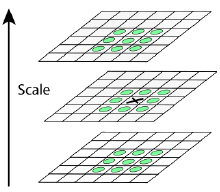
\includegraphics[height=.3\textheight]{img/sift-extremum.png}
  \caption{Метод поиска экстремумов.}
  \label{fig:sift-extr} 
\end{figure}

В каждом изображении из пирамиды DoG ищутся точки локального экстремума. Каждая
точка текущего изображения DoG сравнивается с её восьмью соседями и с девятью
соседями в DoG, находящихся на уровень выше и ниже в пирамиде. Если эта точка
больше (меньше) всех соседей, то она принимается за точку локального экстремума.


Для того, чтобы проверить на наличие точек экстремума $N$'e изображение в DoG
пирамиде, нужно иметь $N+1$'е. А для того, чтобы получить $N+1$'е в DoG
пирамиде, надо иметь $N+1$'е и $N+2$'е изображения в пирамиде гауссианов. Следуя
той же логике можно сказать, что нужно строить 0'е изображение (для проверки
1'го) в пирамиде DoG и ещё два в пирамиде гауссианов. Но 1'е изображение в
текущей октаве имеет тот же масштаб, что и $N$'е в предыдущей (которое уже
должно быть проверено).


Рассмотрим уточнение особых точек. Проверяем пригодность точки экстремума на
роль ключевой.


Определяются координаты особой точки с субпиксельной точностью. Это достигается
с помощью аппроксимирования функции DoG многочленом Тейлора второго порядка,
взятого в точке вычисленного экстремума.
\[ D(x) = D + \frac{\partial D^T}{\partial x}x + \frac{1}{2}x^T\frac{\partial^2D}{\partial x^2}x, \]
где $D$ - функция DoG, $X = (x,y,\sigma)$ --- вектор смещения относительно точки
разложения, первая производная DoG --- градиент, вторая --- матрица Гессе.


Экстремум многочлена Тейлора находится путем вычисления производной и
приравнивания ее к нулю. В итоге получим смещение точки вычисленного экстремума,
относительно точного
\[ \widehat{x} = -\frac{\partial^2D^{-1}}{\partial x^2}\frac{\partial D}{\partial x}. \]

Все производные вычисляются по формулам конечных разностей. В итоге получаем
СЛАУ размерности $3 \times 3$, относительно компонент вектора $\widehat{x}$.


Если одна из компонент вектора $\widehat{x}$ больше половины шага сетки в этом
направлении, то это означает, что на самом деле точка экстремума была вычислена
неверно и нужно сдвинуться к соседней точке в направлении указанных
компонент. Для соседней точки все повторяется заново. Если таким образом мы
вышли за пределы октавы, то следует исключить данную точку из рассмотрения.


Когда положение точки экстремума вычислено, проверяется на малость само значение
DoG в этой точке по формуле
\[ D(\widehat{x}) = D + \frac{1}{2}\frac{\partial D^T}{\partial x}\widehat{x}. \]

Если последняя проверка не проходит, то точка исключается, как точка с малым
контрастом.


Строим гистограмму ориентаций $\theta(x,y)$
\[m(x,y) = \sqrt{((L(x+1),y) - L(x-1,y))^2 + (L(x,y+1)-L(x,y-1))^2}, \]
\[\theta(x,y) = tanh(L(x,y+1) - L(x,y-1) / (L(x+1,y) - L(x-1,y)). \]

Вычисляем дескрипторы ключевых точек. Далее дескриптор локальных
особенностей вычисляется для каждой ключевой точки. Он основан на локальном
градиенте изображения, трансформированном в соответствии с ориентацией ключевой
точки, чтобы предоставить неизменность ориентации. Каждая особенность --- это
вектор с размерностью 128 явно идентифицирующий окрестности ключевой точки.


Дескриптор каждой ключевой точки, вычисленной для нового изображения лица,
независимо сравнивается с сохраненными дескрипторами ключевых точек лиц, и при
достаточном совпадении считаем, что лица совпадают.

\paragraph{Преимущества:}
\begin{enumerate}
\item более высокие показатели распознавания по сравнению с холистическими
методами (PCA, LDA);
\item инвариантность метода к масштабу.
\end{enumerate}

\paragraph{Недостатки:}
\begin{enumerate}
\item на лице человека обычно слишком мало углов, для которых определяются
ключевые точки;
\item запатентован в США, что делает невозможным коммерческое использования без
получения разрешения автора.
\end{enumerate}

% +
\subsubsection{Метод локальных бинарных шаблонов} 
Изначально оператор LBP \cite{LBP} был создан для описания текстуры. Оператор
сопоставляет каждому пикселю 8-битное значение, вычисляемое в зависимости от
значений интенсивностей рассматриваемого пикселя и его 8-ми соседей, как
показано на рисунке \ref{fig:lbp-operator}. Затем гистограммы таких значений
различных регионов лица могут быть использованы в качестве дескриптора текстуры
лица.


Локальные бинарные шаблоны вычисляются путем применения определенного оператора
к каждому пикселю изображения. Этот оператор работает следующим образом. Вначале
значение интенсивности в пикселе сравнивается со значениями во всех пикселях из
некоторой окрестности, например, размером 3×3 пикселя. Результат сравнения
записывается как 0, если значение рассматриваемого пикселя меньше центрального,
и как 1 в противном случае. Для рассматриваемой окрестности 3 на 3 получается 8
цифр, из которых составляется двоичный вектор, который интерпретируется как
двоичная запись целого числа. Это число и является результатом применения
оператора к пикселю. Итоговые признаки получаются после разбиения всего
изображения решеткой на прямоугольные области, подсчета гистограмм частот
появления чисел в каждой области и конкатенации гистограмм по всем областям в
один вектор. Процесс вычисления локальных бинарных шаблонов показан на рисунке
\ref{fig:lbp-operator}.

\begin{figure}[h!]  \centering
  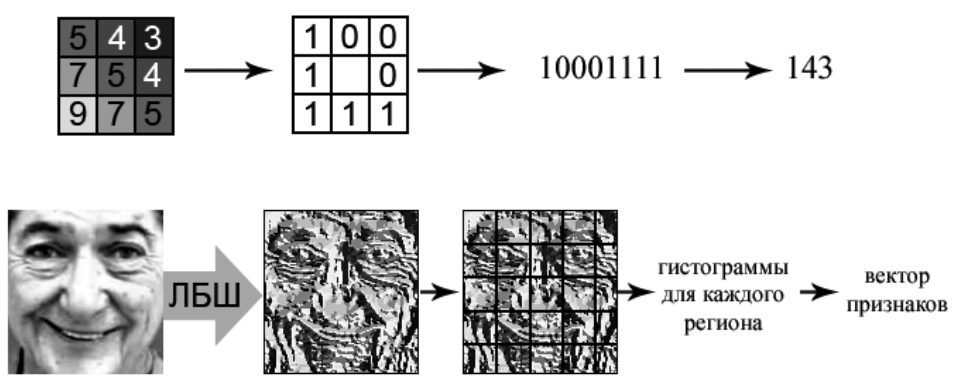
\includegraphics[width=0.6\textwidth,height=.2\textheight]{img/lbp-operator.png}
  \caption{Вычисление локальных бинарных шаблонов: вверху – для одного пикселя,
внизу – для целого изображения.}
  \label{fig:lbp-operator}
\end{figure}

Признаки, полученные таким образом, устойчивы к небольшим изменениям
освещенности и небольшим сдвигам в положении лица \ref{fig:lbp-faces}. Эта
устойчивость достигается за счет того, что подсчет ведется не индивидуально для
каждого пикселя, а используются области значительного размера.

\begin{figure}[h!]  \centering
  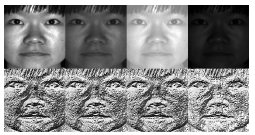
\includegraphics[width=0.55\textwidth,height=.2\textheight]{img/lbp-faces.jpg}
  \caption{Пример использования оператора lbp для изображений лиц с различной
степенью освещенности.}
  \label{fig:lbp-faces}
\end{figure}

Более формально оператор LBP можно описать так:
\[ LBP(x_C,y_c) = \sum_{p=0}^{p-1}2^ps(i_p-i_c),\] где $(x_c,y_c)$ ---
координаты центрального пикселя с интесивностью $i_c$; $i_n$ --- интенсивность
соседнего пикселя, а s --- функция, определенная следующим образом:
\[ s(x) = \begin{cases} 1, \mbox{если $x \geq 0$} \\ 0, \mbox{иначе}
          \end{cases}
\]

В скором времени было обнаружено, что данный оператор не может закодировать
детали в различном масштабе. Тогда данный оператор был расширен, чтобы
использовать произвольные соседние пиксели. Идея заключается в том, чтобы задать
радиус отступа от рассматриваемого до интересующих нас пикселей и количество
пикселей-соседей. Для рассматриваемой точки $(x_p,y_p)$ позиция соседа
$(x_p,y_p),p \in P$ может быть вычислена так:
\[ x_p = x_c + R\cos(\frac{2\pi p}{P}) \]
\[ y_p = y_c - R\sin(\frac{2\pi p}{P}), \] где R --- радиус
окружности(расстояние от рассматриваемого пикселя до соседей), а P ---
количество рассматриваемых соседей.


Такой оператор является расширением оригинального LBP, так что он называется
расширенным LBP (Extended LBP) либо круговым LBP (Circular LBP). Если координата
точки на окружности не совпадает с координатой на изображении, можно получить
координаты точки с помощью интерполяции. Например, билинейной:
\[ f(x,y) \approx 
\begin{bmatrix} 1 - x & x
\end{bmatrix}
\begin{bmatrix} f(0,0) & f(0,1) \\ f(1,0) & f(1,1)
\end{bmatrix}
\begin{bmatrix} 1 - y \\ y
\end{bmatrix}
\]


Из рисунка \ref{fig:lbp-operator} можно увидеть, что процесс выделения признаков
из изображения с помощью оператора LBP состоит из следующих шагов:
\begin{enumerate}
\item выбрать количество регионов, на которые будем делить изображение;
\item выбрать радиус окружности и количество точек, участвующих в рассмотрении,
если используется оператор Расширенный LBP;
\item разделить изображение, посчитать гистограммы количества одинаковых
значений оператора, примененного для каждого пикселя области, для каждой
области;
\item соединить их в результирующий вектор, который и будет представлять наше
изображение.
\end{enumerate}

\subsection{Анализ качества распознавания различных методов} Результаты
сравнения будут приведены согласно \cite{Comparison}. Было получено 10
предобработанных изображений 110 объектов, затем они были сжаты, используя
пирамиду Гаусса. После чего были подготовлены уровни Гаусса. Уровень 1 содержит
изображения 100x100 пикселей, уровень 2 --- 50x50, 3 --- 25x25, 4 --- 13x13, 5
--- 7x7.


В таблице \ref{tab:6x4} шесть изображений из каждого набора составляли базу данных, а 4 были тестовыми.

\begin{table}[h!]
  \begin{tabu}{|X|l|l|l|l|l|}\hline
    60/40\% \linebreak Галерея/Пробные & Уровень 1 & Уровень 2 & Уровень 3 & Уровень 4 & Уровень 5 \\\hline
    PCA & 71.5 & 72 & 71 & 71 & 51\\\hline
    LDA & 76.5 & 73 & 75 & 72.5 & 48.5\\\hline
    SIFT & 81 & 80 & 80 & 78 & 61\\\hline
    LBP & 78.6 & 78 & 78 & 77.2 & 60\\\hline
  \end{tabu}
  \caption{Галерея/Пробные - 60/40 \%}
  \label{tab:6x4}
\end{table}

В таблице \ref{tab:8x2} восемь изображений из каждого набора составляли базу данных,
а 2 были тестовыми.

\begin{table}[h!]
  \begin{tabu}{|X|l|l|l|l|l|}\hline
    80/20\% \linebreak Галерея/Пробные & Уровень 1 & Уровень 2 & Уровень 3 & Уровень 4 & Уровень 5 \\\hline
    PCA & 75 & 75 & 79 & 83 & 56\\\hline
    LDA & 77 & 77 & 83 & 82 & 58\\\hline
    SIFT & 81 & 83 & 82 & 80 & 70\\\hline
    LBP & 81.3 & 81 & 82.5 & 80 & 61\\\hline
  \end{tabu}
  \caption{Галерея/Пробные - 80/20 \%}
  \label{tab:8x2}
\end{table}

\subsection{Классификация}
Классификацию предполагается производить с помощью нейронной сети,
обучаемой методом обратного распространения ошибки, так как данный метод
классификации предоставляет широкий спектр настроек (подбор коэффициентов) и
делает возможным последующие улучшения, например построение сети глубокой
архитектуры.

% +
\subsection{Вывод}
В данном эксперименте участвовали изображения, на которых лица были оптимально
освещены, но и тут LBP опережает PCA и LDA. SIFT несколько опережает LBP, во
многом благодаря условиям освещения. Также скорость работы SIFT значительно
уступает скорости работы LBP, исходя из описания алгоритмов.


Благодаря скорости работы, независимости от условий освещения и приемлемой
точности распознавания был выбран метод локальных бинарных шаблонов(LBP).

% -
\section{Конструкторский раздел}
\subsection{Конвертация изображения} В качестве метода для представления
изображения, как информации для последующей классификации, был выбран метод
локальных бинарных шаблонов. Данный метод был выбран за его репрезентативные
возможности, независимость от условий освещенности, приемлемые показатели
распознавания, высокую скорость работы, простоту реализации и возможность
распараллеливания вычислений.


На данном шаге алгоритма на вход поступает вектор с обучающей выборкой, который
содержит изображения в формате градаций серого. Вынимаем поочередно изображения
и к каждому попиксельно применяем оператор локальных бинарных шаблонов, затем
формируем новый вектор, который содержит строки с информацией об
изображениях. Данный вектор впоследствии передается на вход следующему шагу
алгоритма.


Когда нам необходимо распознать, кому принадлежит изображение, мы также
попиксельно обрабатываем его оператором локальных бинарных шаблонов, а затем
передаем обученному классификатору.

\subsection{Классификация} В качестве классификатора была выбрана нейронная
сеть. Нейронная сеть представляет собой упрощенную математическую модель нервной
системы живых существ, в частности, головной мозг человека. Была выбрана сеть с
прямым распространением сигнала. Определение сети и алгоритм её обучения будут
представлены согласно \cite{Statistical_Methods}.


Нейронная сеть прямого распространения - это связный ориентированный
ациклический граф с множеством вершин $V = \{v_1,\dots,v_S\}$ (рецепторов и
нейронов) и ребер (синапсов) $E = {e_1,\dots,e_T}$, снабженный следующей
дополнительной структурой:
\begin{enumerate}
\item множества вершин-истоков (рецепторов) $V_{in}$ и вершин-стоков (выходных
нейронов) $V_{out}$ нейронной сети (непустые, как у всякого связного
ориентированного ациклического графа) упорядочены;
\item каждому ребру $e$ приписан параметр $w_e \in \Re$ и функция $f_e:\Re^2 \to
\Re$, называемая функцией проводимости ребра (синапса);
\item каждой вершине $v \in V \ V_{in}$ приписан параметр $w_v \in \Re$ и
функция $g_v:\Re^2 \to \Re$, называемая функцией активации вершины (нейрона).
\end{enumerate}

Упорядоченные множества $V_{in} = (v_{in}^1,\dots,v_{in}^d)$ и $V_{out} =
(v_{out}^1,\dots,v_{out}^q$ содержат $d$ и $q$ вершин, соответственно. Нейронная
сеть вычисляет вектор-функции $f : \Re^d \to \Re^q$ , зависящие также от
параметров всех вершин и ребер сети. Для вычисления значения $y = f (x)$ на
вершинах и ребрах сети определяется вспомогательная вещественнозначная функция u
(потенциал), зависящая от вектор-аргумента $x$ и параметров сети $w$, причем
потенциал $u(e)$ каждого ребра e равен потенциалу $u(v)$ вершины $v$, из которой
это ребро выходит $(e \in V_{out})$. Потенциал определяется индуктивно:
\begin{enumerate}
\item потенциал j-го источка $v_{in}^j$ равен j-му аргументу $x^j$,
т.е. $u(v_{in}^j = x^j$;
\item для каждой вершины $v$, для всех входящих ребер которой входные потенциалы
уже определены, вычисляется активирующая сумма
\[ s(v) = \sum_{e \in v_{in}} h_e(w_e,u(e)) \] и потенциал
\[ u(v) = g_v(w_v,s(v)) .\]
\end{enumerate}

Связность и ацикличность сети гарантируют корректное вычисление потенциала
каждой вершины. Результатом вычисления является вектор-потенциал $y =
(y^1,\dots,y^q) = (u(v_{out}^1),\dots,u(v_{out}^q))$ вершин-стоков.


Вектор $w$, составленный из всех чисел $w_e$ и $w_v$ , является параметром
сети. Обучение нейронной сети заключается в подборе такого значения $w$, чтобы
выходной вектор $y$, являющийся функцией $y = f(x) = F(w, x)$ от параметра и
входного вектора $x$, был похож на то, чему сеть пытаются научить. Наоборот,
функции $h_e$ и $g_v$ и сам ориентированный граф остаются неизменными.


Для простоты и удобства реализации нейронной сети обычно полагают ее состоящей
из нейронов нескольких (немногих) разновидностей, регулярным образом соединенных
друг с другом. Чаще всего множество $V$ всех нейронов сети предполагаются
разбитым на пронумерованные слои $V_0 = V_{in}, V_1,\dots,V_L = V_{out}$, так
что
\begin{enumerate}
\item каждое ребро, входящее в нейрон некоторого i-го слоя, выходит из некторого
нейрона (i-1)-го слоя;
\item для каждого слоя функции активации $g_v$ всех нейронов этого слоя
совпадают; совпадают и функции проводимости $h_e$ всех входящих в них ребер.
\end{enumerate}

Такая нейронная сеть называется L-слойной. Послойная градуировка автоматически
обеспечивает ацикличность сетей. В практически применяемых нейронных сетях
послойная структура может быть более сложной и не вполне регулярной.


Наиболее типичными для многослойных сетей являются следующие функции
проводимости ребер и активации нейронов:
\begin{enumerate}
\item $h_e(w_e,u) = w_eu$, а $g_v(w_v,s) = th(s - w_v)$ (гиперболический тангенс
разности), $g_v(w_v,s) = \sigma(s-w_v)$ (логическая функция от разности), или
какое-нибудь другое гладкое монотонно возрастающее приближение ступенчатой
функции;
\item $h_e(w_e,u) = (u - w_e)^2$, а $g_v(w_v,s) = e^{-s/2w_v}$ или какое -нибудь
другое гладкое приближение дельта-функции.
\end{enumerate} Функция активации выходных нейронов (нейронов последнего слоя)
обычно определяется задачей, для решения которой нейронная сеть предназначена.


Искусственные нейронные сети могут применяться для вычисления функций как от
дискретных, так и от непрерывных признаков. В последнем случае для устойчивости
сети к ошибкам измерения входных векторов необходима непрерывность функций $h_e$
и $g_v$ , а для обучения сети градиентными методами — еще и их
дифференцируемость. В дальнейшем функции $h_e$ и $g_v$ предполагаются гладкими.


Количество L слоев в практически применяемых нейронных сетях на удивление мало:
чаще всего встречаются трехслойные сети, иногда даже двухслойные. И наоборот, в
одном и том же распознавании иногда участвуют несколько различных сетей, как-то
соединенных друг с другом, но обучаемых раздельно. Сеть может и не иметь никакой
регулярной многослойной структуры.


Количество $d$ входов искусственной сети и количество $q$ ее выходных нейронов
определяются решаемой задачей и обычно не очень велики. $d$ равно размерности
пространства признаков (обычно десятки или сотни), а $q$ меняется от 1
(регрессия) до сотен (многоклассовая классификация). Наоборот, число остальных
нейронов, называемых скрытыми, бывает порядка тысяч и десятков тысяч, а число
ребер доходит до миллионов, хотя это несравнимо меньше, чем в естественной
нейронной сети. В искусственных нейронных сетях, как и в мозгу, все вычисления
могут происходить параллельно, и тем самым, очень быстро. В реальности нейронные
сети моделируются на обычных последовательных компьютерах и работают не слишком
быстро, а главное, медленно обучаются, поэтому на количестве вершин и ребер сети
приходится экономить. Появляющиеся время от времени аппаратные реализации
нейронных сетей (нейрокомпьютеры) позволяют несколько увеличить размеры
пригодных для обучения сетей.


Создание нейронной сети для решения какой-либо задачи состоит из двух этапов:
построение сети, т.е. ациклического ориентированного графа и функций
проводимости и активации, и подбор ее параметров w. Первый этап — очень
эвристический и существенно зависящий от конкретной решаемой задачи и объема
доступных обучающих данных, и как правило требует многочисленных
экспериментов. Для второго этапа — обучения — применяются довольно универсальные
методы.


Типичный распознающий перцептрон — трехслойный. Нейроны первого скрытого слоя
разбиты на несколько групп: внутри каждой группы нейроны одинаковы и соединены
не со всеми входами сети, а только с каким-то их подмножеством, своим для каждой
группы. Это разбиение на группы производится вручную исходя из специфики
задачи. Например, при распознавании растровых изображений каждый нейрон первого
слоя может иметь свое небольшое “поле зрения”, т.е. быть соединенным с
рецепторами, измеряющими яркость изображения в некотором количестве (нескольких
десятках) смежных точек. Поля зрения разных нейронов одной группы сдвинуты друг
относительно друга (обычно поля зрения “соседних” нейронов перекрываются), а
нейроны разных групп имеют разные по размеру и по форме поля зрения. Нейроны
второго скрытого слоя более-менее одинаковы, но каждый нейрон соединен со
случайным не слишком большим подмножеством нейронов первого слоя. Каждый нейрон
третьего слоя (выходного) соединен со всеми нейронами второго слоя.

\paragraph{Обучение многослойного перцептрона: метод обратного распространения ошибки (error back-propagation).}
Обучение перцептрона, вычисляющего функцию F(w,x) --- это поиск вектора весой и
смещений w, минимзирующего регуляризованную суммарную ошибку
\[ E_T(w) = \phi(w) + \sum_{i=1}^NE(F(w,x_i),y_i) \]
на некотором обучающем наборе $T = ((x_1,y_1),\dots,(x_N,y_N))$. Обучение чаще
всего производится методом градиентного спуска и комбинированием его с другими
методами. Для его применимости функции активации всех нейронов и функции ошибки
$E$ и регуляризации $\phi$ должны быть дифференциируемы. Вычисление градиента не
совсем просто из-за огромной размерности параметра $w$ и отсутствия явных формул
для производных функции $F$ по $w$.


Замечательно то, что этот огромной размерности градиент ошибки по параметру для
нейронной сети можно вычислять красиво и быстро — за время того же порядка, что
и время работы сети — с помощью другой (двойственной) нейронной сети,
получающейся из исходной обращением направлений ребер. На этом основании
градиентный спуск для нейронных сетей обычно называется не просто градиентным
спуском, а методом обратного распространения ошибки. Хотя строго говоря, метод
обратного распространения — это всего лишь способ вычисления градиента ошибки, и
даже не обязательно ошибки, а любой функции от выхода нейронной
сети. Конфигурация двойственной сети однозначно определена конфигурацией
исходной сети, а веса и функции активации зависят от весов ребер исходной сети и
набора значений $\{u(v)\}$ потенциалов нейронов. А именно,
\begin{enumerate}
\item нейронами $\breve{v}\dots$ двойственной сети являются все скрытые нейроны
и входы $v\dots$ исходной сети;
\item входами $\breve{v}_L^1,\dots,\breve{v}_L^q$ двойственной сети являются
выходные нейроны исходной сети;
\item ребрами $\breve{e}\dots$ двойственной сети являются ребра $e\dots$
исходной сети с обращенными направлениями;
\item каждому ребру двойственной сети $\breve{e}$ приписан вес
$\breve{w}_{\breve{e}} = w_e$, где $e$ --- ребро-двойник $\breve{e}$; каждому
скрытому нейрону двойственной сети $\breve{v}$ приписана функция активации
$\breve{g_{\breve{v}}}$, являющаяся умножением на $g'_v(g_v^{-1}(u(v))) =
g'_v(s(v) - w_v)$, т.е. на производную функции активации $g_v$ двойника $v$
нейрона $\breve{v}$ в исходной сети, взятую в прообразе значения $u(v)$
относительно $g_v$, а каждому выходному нейрону --- тождественная функция
активации.
\end{enumerate} Таким образом, двойственная сеть зависит не только от исходной
сети, но и от поданного на нее входного вектора.

\subsection{Схема алгоритма распознавания}

На рисуне \ref{fig:alg} отображены основные шаги алгоритма распознавания. Перед
началом работы алгоритма входные данные должны быть предобработаны, а именно:
изображения должны быть преобразованы в режим градаций серого.

\begin{figure}[h!]
  \centering
  \includegraphics[width=.4\textwidth,height=.8\textheight]{img/algorithm.eps}
  \caption{Схема алгоритма распознавания.}
  \label{fig:alg}
\end{figure}

\section{Технологический раздел}

\subsection{Технические средства}

\subsubsection{Язык программирования}
Для разработки был выбран язык программирования C++. Из его достоинств следует
выделить высокую скорость (практически сравнимую с языком C для современных
компиляторов) и широкие возможности, позволяющие достаточно писать достаточно
удобный и выразительный код по сравнению с тем же C, а так же вероятно самое
большое количество удобных сторонних библиотек на все случаи жизни. Также C++
предоставляет громоздкие, но крайне эффективные методы шаблонного
метапрограммирования, позволяющие генерировать очень эффективный код из
неповторяющихся блоков. Из недостатков следует выделить сложность синтаксиса и
большое количество правил языка и нетривиальных моментов в языке, из чего
следует потенциально большое количество скрытых ошибок.

Было выбрано подмножество языка C++11, которое даёт разработчику новые
возможности по написанию более быстрого и понятного кода, большие приятные
нововведения в библиотеку C++ STL, а так же новые конструкции для избавления от
некоторых ошибок.

В качестве альтернатив рассматривались некоторые функциональные языки
программирования (Haskell, Racket), скриптовые языки общего назначения с
привязками к библиотекам с машинным кодом (Python, Ruby), языки общего
назначения со сборкой мусора, исполняемые на виртуальной машине (Java,
Scala). Поскольку проект предполагает громоздкие вычисления с необходимостью
расчётов в реальном времени, был сделан выбор в пользу компилируемых в машинный
код языков программирования, среди которых был выбран C++ как наиболее удобный и
функциональный, а также как один из самых быстрых.  На момент начала работы
основные аспекты языка уже были изучены, что позволило целиком
сконцентрироваться на задаче, а не тратить время на изучения инструмента.

\subsubsection{Компилятор}
В процессе разработки использовались два компилятора языка C++: GNU G++ и
CLang. Первый представляет из себя самый развитый и популярный свободный
компилятор для языка C++ в мире, включает в себя большое множество оптимизаций,
поддерживаемых платформ и генерирует крайне эффективный код. Второй, также
свободный, компилятор использовался для анализа кода, так как генерирует
превосходные сообщения об ошибках и обнаруживает некоторые спорные моменты,
которые ``обходит стороной'' G++. Оба компилятора были выбраны по соображениям
большого количества поддерживаемых платформ, в том числе Linux, на котором в
основном разрабатывался данный проект.

\subsubsection{Утилиты и среды разработки}
Проект разрабатывался в нескольких средах разработки. В основном разработка
делилась на два цикла --- написание кода и отладка. Для написания кода
использовался расширяемый текстовый редактор GNU/Emacs с набором расширений, обеспечивающих
предельно комфортную работу с исходным кодом на языке C++. Для сборки и отладки
использовась IDE Qt Creator, которая предоставляет удобный интерфейс к крайне
функциональному и мощному отладчику GNU GDB, позволяет открывать проекты,
написанные с использованием системы сборки CMake и в целом комфортна для
работы. Альтернативами приведённым инструментам является текстовый редактор
Vim и интерфейс отладчика GDB CGDB, предоставляющий консольный
псевдo-оконный интерфейс для работы.

\subsubsection{Поиск ошибок}
В процессе разработки использовался свободный кроссплатформенный отладчик GNU
GDB, предоставляющий широкие возможности по отслеживанию выполнения программы,
поиску ошибок и изучению её работы. Также в процессе разработки использовался
статический анализатор кода CppCheck, указывающий на множество незамеченных и
неочевидных ошибок в исходном коде на основе его анализа. Для поиска ошибок
выделения памяти использовался анализатор памяти Valgrind, результатом работы
которого является список потенциальных утечек памяти, использований
освобождённой памяти и других ошибок работы с ней. Для измерения скорости работы
частей программы и нахождения узких мест использовался комплекс для измерения
производительности Valgrind, предоставляющий табоицу функций программы со
множеством статистических и временных данных.

\subsubsection{Основная библиотека}
В качестве основной библиотеки для работы с изображениями используется opencv,
являющаяся библиотекой алгоритмов компьютерного зрения, обработки изображений и
численных алгоритмов общего назначения с открытым исходным кодом. Она
реализована на C++,что позволило просто интегрировать ее в код
проекта. Также данная библиотека может свободно использоваться и в академических
и в коммерческих целях.


При реализации нейронной сети была использована библиотека eigen. Eigen —
библиотека линейной алгебры для C++ с открытым исходным кодом. Написана на
шаблонах и предназначена для векторно-матричных вычислений и связанных с ними
операций. Eigen характеризуется простым API и высокой производительностью.

\subsubsection{Тестирование}
Для написания тестов был использован Google C++ Testing Framework, который
является библиотекой для модульного тестирования на языке \verb!C++!. Google
Test построена на методологии тестирования xUnit, то есть когда отдельные части
программы (классы, функции, модули) проверяются отдельно друг от друга, в
изоляции.

% + 
\subsubsection{Сборка и запуск разработанного программного обеспечения}
Проект собирался при помощи системы сборки проектов CMake. Она была выбрана
из-за большой гибкости, простоты подключения и линковки сторонних библиотек и
удобства и относительной простоты файлов описания процесса сборки.

Для сборки разработанного программного обеспечения необходимо склонировать
репозиторий с исходным кодом или скопировать папку с ним к себе на ПК. После
чего необходимо установить библиотеку opencv c файлами для разработчиков, а
затем запустить cmake.

\subsubsection{Документация}
С помощью утилиты Doxygen были сгенерированы диаграммы, отображающие
взаимосвязи исходного кода. Это позволяет ``увидеть'' архитектуру,
не читая все исходные файлы проекта.

\subsubsection{Сопроводительные записки}
Техническое задание, расчётно-пояснительная записка и прочее верстались
используя систему вёрстки \LaTeX . Это дало возможность сконцетрироваться на
тексте вместо его оформления, получая красивую вёрстку ``из коробки'', множество
удобных средств для оформления текста и прочее.

\subsection{Формат конфигурационного файла}
При запуске разработанного приложения ему через интерфейс командной строки
передается имя файла в формате csv, который содержит пути к изображениями. В
данном файле последнее изображение является тестовым, а все остальные ---
обучающей выборкой. Формат строки в файле: /путь/к/файлу;метка. Метка содержит
идентификационный номер человека, которому принадлежит изображение.


Изображения хранятся в папках, каждая из которых принадлежит одному
человеку. Был написан скрипт на языке python, генерирующий данный csv файл. Для
запуска ему нужно передать путь к корневой папке, содержащей персональные папки
с изображениями. Формат изображений: 92 пикселя в ширину на 112 пикселей в
высоту.


На выходе алгоритм печатает в стандартный поток вывода предполагаемый класс,
которому принадлежит изображение.

\subsection{Модульное тестирование}
Для разработанного программного обеспечения были написаны модульные тесты,
позволяющие проверить корректность ранее оттестированного кода при внесении
изменений. Пример прогонки модульных тестов показан на рисунке
\ref{fig:test}. Пример исходного кода модульных тестов представлен в приложенни
\ref{ap1}.

\begin{figure}[h!]
  \centering
  \includegraphics[width=.6\textwidth]{img/test.png}
  \caption{Пример прогона модульных тестов.}
  \label{fig:test}
\end{figure}

\subsection{Структура программы}
Здесь мы опишем структуру программы, её основные элементы и устройство.
На рисунке \ref{fig:proj-struct} увидеть из каких модулей состоит программа.

\begin{figure}[h!]
  \centering
  \includegraphics[height=.3\textheight,width=\textwidth]{img/project_structure.png}
  \caption{Структура программы.}
  \label{fig:proj-struct}
\end{figure}

\subsubsection{Оператор локальных бинарных шаблонов}
В программе используется функция, реализующая оператор локальных бинарных
шаблонов. Она позволяет изменять количество регионов изображения, для 
которых считаются гистограммы. Также она позволяет изменять радиус
``осмотра'' и количество ``рассматриваемых соседей''.

\subsubsection{Нейронная сеть}
Был реализован класс нейронной сети, позволяющий смоделировать
многослойную нейронную сеть. В качестве параметров при создании можно
указать количество слоев, количество нейронов в каждом из них, а также
``пороговую'' функцию.


На рисунке \ref{fig:ann-uml} можно увидеть uml диаграмму класса нейронной сети,
из которого видно, что сеть имеет 3 существенных публичных метода: 
создать (Create), тренировать (Train) и предсказать (Predict). Из публичных 
методов можно выделить: инициализацию весов (InitializeWeights), рассчитать
выходы (FeedForward), обновить веса (UpdateBackpropagation). Нейронная сеть
спроектирована так, чтобы ее можно было легко изменить или расширить.
Можно применить наследование и, переписав необходимые методы, поулчить желаемую
реализацию вместо существующей.

\begin{figure}[h!]
  \centering
  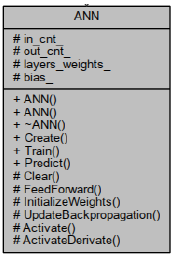
\includegraphics[height=.4\textheight,width=.4\textwidth]{img/ann.png}
  \caption{UML диаграмма класса нейронной сети.}
  \label{fig:ann-uml}
\end{figure}

%\subsubsection{Интерфейс}

\section{Экспериментальный раздел}
\subsection{Достоверность распознавания}
Целью экспериментов является определение достоверности распознавания
разработанным программным продуктом. Достоверность распознавания определяется по
формуле
\[ \frac{TP}{TP+FP}, \]
где $TP$ - число правильно определенных объектов, $FP$ - число ложных обнаружений.


В эксперименте учавствуют 400 изображений, принадлежащие 40 людям.  Одно из
десяти изображений, принадлежащих одному человеку, является тестовым и не входит
в обучающую выборку.  В ходе экспериментов были получены результаты тестирования
скорости и достоверности распознавания. Результаты представлены на рисунке
\ref{fig:acc}.

\begin{figure}[h!]
  \centering
  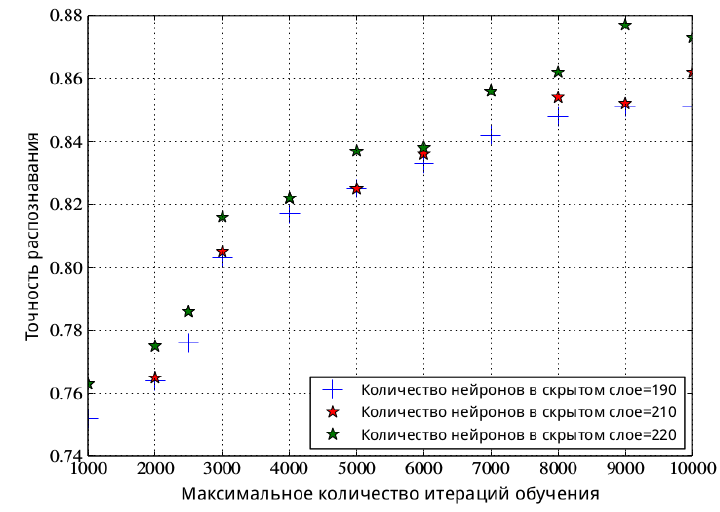
\includegraphics[height=.5\textheight,width=\textwidth]{img/acc_from_iter.png}
  \caption{Исследование достоверности распознавания в зависимости от числа
максимальных итераций обучения нейронной сети.}
  \label{fig:acc}
\end{figure}

\subsection{Скорость распознавания}
Также были проведены исследования скорости обучения нейронной сети
в зависимости от максимального количества итераций. Результаты представлены на
рисунке \ref{fig:time}.

\begin{figure}[h!]
  \centering
  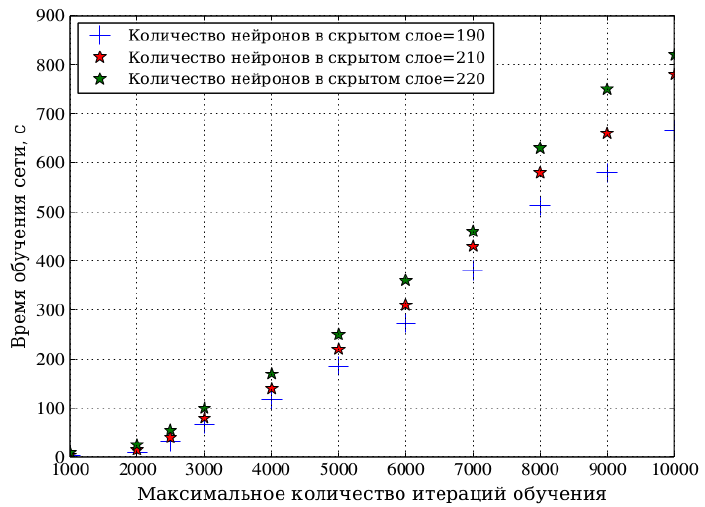
\includegraphics[height=.5\textheight,width=\textwidth]{img/time_from_iter.png}
  \caption{Исследование времени обучения в зависимости от числа максимальных 
итераций обучения нейронной сети.}
  \label{fig:time}
\end{figure}

% remove
\newpage
\section{Организационно-экономическая часть}
\subsection{Введение}
Заказчиком (кафедрой) сформулировано техническое задание на разработку ПП.

Необходимо разработать ПП, осуществляющий распознавание лиц в реальном времени с
приемлемой точностью.
	
Данный проект выполнен в среде Emacs. Заказчик предполагает реализовывать ПП на
электронном информационном носителе (компакт-диске).

На рынке подобные продукты представлены как бесплатными продуктами (OpenCv,
PCL), так и коммерческими продуктами (Синезис).


Расчёты производились в соответствии с \cite{OIPP}.

\subsection*{Организация и планирование процесса разработки}
При использовании традиционного подхода, организация и планирование процесса
разработки программного продукта или программного комплекса предусматривает
выполнение следующих работ:

\begin{itemize}
\item формирование состава выполняемых работ и группировка их по стадиям
разработки;
\item расчет трудоемкости выполнения работ;
\item установление профессионального состава и расчет количества исполнителей;
\item определение продолжительности выполнения отдельных этапов разработки;
\item построение календарного графика выполнения разработки;
\end{itemize}

Планирование длительности этапов и содержания проекта осуществляется в
соответствии с ЕСПД ГОСТ 34.603-92 и распределяет работы по этапам, как показано
в таб.~\ref{tab:econ-stages}
\begin{table}
  \begin{tabu}{|c|c|X[l]|}\hline
    Основные стадии & № & Содержание работы \\\hline
    \multirow{2}{*}{Техническое задание} & 1 & Постановка задачи \\\cline{2-3}
         & 2 & Выбор средств разработки и реализации \\\hline
    \multirow{2}{*}{Эскизный проект} & 3 & Разработка математической модели \\\cline{2-3}
         & 4 & Разработка алгоритмов расчёта задачи \\\hline     
    \multirow{2}{*}{Техно-рабочий проект} & 5 & Реализация алгоритмов расчёта задачи \\\cline{2-3}
         & 6 & Разработка пользовательского интерфейса \\\cline{2-3}            
         & 7 & Реализация пользовательского интерфейса \\\hline
    Внедрение & 8 & Проведение вычислительных экспериментов \\\hline
  \end{tabu}
  \caption{Распределение работ по этапам.}
  \label{tab:econ-stages}
\end{table}

\subsection*{Расчёт трудоёмкости выполнения работ}
Трудоемкость разработки программной продукции зависит от ряда
факторов, основными из которых являются следующие:
\begin{itemize}
  \item степень новизны разрабатываемого программного комплекса,
  \item сложность алгоритма его функционирования,
  \item объем используемой информации, вид ее представления и способ обработки,
  \item уровень используемого алгоритмического языка программирования
\end{itemize}

Исходные данные расчета приведены в табл.~\ref{tab:econ-init}.

\begin{table}[H]
  \begin{tabu}{|X[l]|>{\centering}m{1.5cm}|X[l]|}\hline
    Функциональное назначение ПП & & Задачи расчётного характера \\\hline
    Алгоритм разработки ПП & 2в &  \\\hline
    Группа новизны & В & Разработка программной продукции, имеющей аналоги \\\hline
    Степень сложности & 1-я группа & Программная продукция, реализующая оптимизационные и моделирующие алгоритмы \\\hline
	По виду представления исходной информации & Группа 12 & Форматный контроль информации. \\\hline
  \end{tabu}
  \caption{Исходные данные}
  \label{tab:econ-init}
\end{table}

Трудоемкость разработки программной продукции $\tau_{ПП}$ может быть определена
как сумма величин трудоемкости выполнения отдельных стадий разработки ПП из
выражения:

\begin{equation}
	\tau_{ПП} = \tau_{ТЗ} + \tau_{ЭП} + \tau_{ТП} + \tau_{РП} + \tau_{В} 
\end{equation}

где 
\begin{itemize}
  \item $\tau_{ТЗ}$ - трудоемкость разработки технического задания на создание ПП;
  \item $\tau_{ЭП}$ - трудоемкость разработки эскизного проекта ПП;
  \item $\tau_{ТП}$ - трудоемкость разработки технического проекта ПП;
  \item $\tau_{РП}$ - трудоемкость разработки рабочего проекта ПП;
  \item $\tau_{В}$ - трудоемкость внедрения разработанного ПП.
\end{itemize}

Трудоемкость разработки технического задания рассчитывается по формуле:
\begin{equation}
	\tau_{ТЗ} = Т_{ЗРЗ} + Т_{ЗРП}
\end{equation}
где 
\begin{itemize}
  \item $Т_{ЗРЗ}$ - затраты времени разработчика постановки задач на разработку ТЗ, чел. дни;
  \item $Т_{ЗРП}$ - затраты времени разработчика программного обеспечения на разработку ТЗ, чел. дни.
\end{itemize}

В расчёте участвуют следующие коэффициенты:
\begin{itemize}
  \item $t_З = 47$ – норма времени на разработку ТЗ на программный продукт в зависимости от функционального назначения и степени новизны разрабатываемого ПП, чел. дни;
  \item $K_{ЗРЗ} = 0,65$ - коэффициент, учитывающий удельный вес трудоемкости работ, выполняемых разработчиком постановки на стадии ТЗ;
  \item $K_{ЗРП} = 0,35$ - коэффициент, учитывающий удельный вес трудоемкости работ, выполняемых разработчиком программного обеспечения на стадии ТЗ.
\end{itemize}

Тогда
\begin{equation}
	\tau_{ТЗ} = 47 (0,65 + 0,35) = 47 \text{ [чел. дни]}
\end{equation}

Аналогично рассчитывается трудоёмкость эскизного проекта ПП $\tau_{ЭП}$:
\begin{equation}
	\tau_{ЭП} = t_{ЭП} (К_{ЭРЗ} + К_{ЭРП}) = 67 (0,75 + 0,25) = 67 \text{ [чел. дни]}
\end{equation}

Трудоемкость разработки технического проекта $\tau_{ТП}$ зависит от функционального назначения ПП, количества разновидностей форм входной и выходной информации и определяется как сумма времени, затраченного разработчиком постановки задач и разработчиком программного обеспечения, т.е.
\begin{gather*}
	\tau_{ТП} = (t_{ТРЗ} + t_{ТРП}) К_В К_р \\
	К_В = (К_П n_П + К_{НС} n_{НС} + К_Б n_Б) / (n_П + n_{НС} + n_Б)
\end{gather*}

где 
\begin{itemize}
  \item $t_{ТРЗ} = 57, t_{ТРП} = 43$ - норма времени, затрачиваемого на разработку технического проекта разработчиком постановки задач и разработчиком ПП соответственно, чел.-дни
  \item $К_Р = 1,26$ - коэффициент учета режима обработки информации
  \item $К_П = 1, К_НС = 0,72, К_Б = 2,18$ - значения коэффициентов учета вида используемой информации для переменной, нормативно-справочной информации и баз данных соответственно
  \item $n_П = 6, n_НС = 4, n_Б = 0$ - значения коэффициентов учета вида используемой информации для переменной, нормативно-справочной информации и баз данных соответственно
\end{itemize}
Тогда 
\begin{gather*}
	\tau_{ТП} = (57 + 43) (1 \cdot 6 + 0,72 \cdot 4 + 2,18 \cdot 0) / (6 + 4 + 0) \cdot 1,26 = 112 \text{ [чел. дни]}
\end{gather*}

Трудоемкость разработки рабочего проекта $\tau_{РП}$ зависит от
функционального назначения ПП, количества разновидностей форм входной
и выходной информации, сложности алгоритма функционирования,
сложности контроля информации, степени использования готовых
программных модулей, уровня алгоритмического языка программирования и
определяется по формуле:
\begin{gather*}
  \tau_{РП} = К_к К_р К_Я К_З К_{ИА} (t_{РРЗ} + t_{РРП})\\
  К_{ИА} = (К_П' n_П + К_{НС}' n_{НС} + К_Б' n_Б) / (n_П + n_{НС} + n_Б)
\end{gather*}
\begin{itemize}
  \item $t_{РРЗ} = 138, t_{РРП} = 979$ - норма времени, затраченного на разработку РП на алгоритмическом языке высокого уровня разработчиком постановки задач и разработчиком программного обеспечения соответственно, чел. дни.
  \item $K_К = 1$ – коэффициент учета сложности контроля информации;
  \item $К_Р = 1,32$ - коэффициент учета режима обработки информации
  \item $K_Я = 1$ – коэффициент учета уровня используемого алгоритмическогоязыка программирования;
  \item $K_З = 0,8$ – коэффициент учета степени использования готовых программных модулей;
  \item $K_{ИА}$ – коэффициент учета вида используемой информации и сложности алгоритма ПП;
  \item $К_П' = 1,20, К_НС' = 0,65, К_Б' = 0,54$ - значения коэффициентов учета сложности алгоритма ПП и вида используемой информации для переменной, нормативно-справочной информации и баз данных соответственно.
\end{itemize}
Тогда
\begin{gather*}
  К_{ИА} = 6 \cdot 1,20 + 4 \cdot 0,65 / (4 + 6) = 0.98 \\
  \tau_{РП} = 1 \cdot 1.32 \cdot 1 \cdot 0,8 \cdot 0,98 \cdot(138 + 979) = 1117 \text{ [чел. дни]}
\end{gather*}

Так как при разработке ПП стадии «Технический проект» и «Рабочий
проект» объединены в стадию «Техно-рабочий проект», то трудоемкость ее
выполнения $\tau_{ТРП}$ определяется по формуле:
\begin{gather*}
  \tau_{ТРП} = 0,85 \tau_{ТП} + \tau_{РП} = 0,85 \cdot 112 + 1117 = 1212 \text{ [чел. дни]}
\end{gather*}

Трудоемкость выполнения стадии внедрения $\tau_{В}$ может быть рассчитана по формуле:
\begin{gather*}
  \tau_{В} = К_к К_р К_З (t_{ВРЗ} + t_{ВРП}) = 1 \cdot 1,32 \cdot 0,8 (33 + 98) = 138 \text{ [чел. дни]}
\end{gather*}

Трудоемкости по этапам разработки проекта представлены в таблице~\ref{tab:econ-trud}.

\begin{table}[H]
  \begin{tabu}{|X[c]|X[c]|}\hline
    Этап & Трудоёмкость этапа, [чел. дни] \\\hline  
    ТЗ & 47 \\\hline  
    ЭП & 67 \\\hline  
    ТРП & 1212 \\\hline  
    В & 138 \\\hline      
    Итого & 1464 \\\hline        
  \end{tabu}
  \caption{Трудоемкости по стадиям разработки проекта}
  \label{tab:econ-trud}
\end{table}

Средняя численность исполнителей при реализации проекта разработки и внедрения ПО определяется соотношением $N = \frac{Q_p}{F}$, 
где
\begin{itemize}
  \item $Q_p = \tau \cdot t_p$ - затраты труда на выполнение проекта (разработка и внедрение ПО),
  \item $F = T \cdot F_M$ - фонд рабочего времени;
  \item $Т$ - время выполнения проекта в месяцах. T = 5 мес.;
  \item $F_M$ - фонд времени в текущем месяце, который рассчитывается из учета общества числа дней в году, числа выходных и праздничных дней и определяется соотношением $F_М = \frac{t_p (D_k - D_B - D_П)}{12}$;
  \item $t_p$ - продолжительность рабочего дня;
  \item $D_K$ - общее число дней в году;
  \item $D_B$ - число выходных дней в году;
  \item $D_П$ - число праздничных дней в году.
\end{itemize}

Тогда 
\begin{gather*}
  F = 5 \cdot 8 (365 - 103 - 13) / 12 = 830\\
  N = 1464 \cdot 8 / 830 = 14 \text{ - число исполнителей проекта.}
\end{gather*}

\subsection*{Календарный план-график}
Планирование и контроль хода выполнения разработки проводится по календарному графику выполнения работ. Планирование процесса разработки и календарный ленточный план представлены в таб. \ref{tab:econ-plan} и рис. \ref{tab:econ-lent} соответственно.

\begin{table}[H]
  \begin{tabu}{|m{2cm}|m{1,5cm}|m{4cm}|m{3cm}|m{1cm}|}\hline
    Стадия & $\tau$ & Должность исполнителя & Распределение трудоемкости & Ч-ть \\\hline
    ТЗ & 47 & \shortstack{Ведущий инженер\\Программист} & \shortstack{37(79 \%)\\10} & \shortstack{1\\1} \\\hline  
    ЭП & 67 & \shortstack{Ведущий инженер\\Программист} & \shortstack{37(55 \%)\\30} & \shortstack{1\\1} \\\hline  
    ТРП & 1212 & \shortstack{Ведущий инженер\\Программист} & \shortstack{81\\13 \times 87} & \shortstack{1\\13} \\\hline  
    В & 138 & \shortstack{Ведущий инженер\\Программист} & \shortstack{38\\2 \times 50} & \shortstack{1\\2} \\\hline      
    Итого & 1464 & & & 14 \\\hline  
  \end{tabu}
  \caption{Планирование процесса разработки.}
  \label{tab:econ-plan}
\end{table}

\begin{figure}[H]
  \centering
  \includegraphics[width=.6\textwidth]{include/timeplan.pdf}
  \caption{Календарный ленточный план работ.}
  \label{tab:econ-lent}
\end{figure}

Вывод: при распараллеливании работы ведущего инженера и
программистов можно добиться сокращения срока разработки и внедрения
программного продукта с 1464 дней до 211 дней, т. е. в 6,94 раза по сравнению
со временем разработки одним человеком.

В таб. \ref{tab:econ-salary} приведены затраты на заработную плату и отчисления
на социальное страхование в пенсионный фонд, фонд занятости и фонд
обязательного медицинского страхования (30\%). Для всех исполнителей
предполагается оклад в размере 20000 рублей в месяц.

\begin{table}[H]
  \centering
  {\tiny
  \begin{tabu}{||c||c|c|c||c|c|c||c|c|c||c|c|c||c||}\hline
   & \multicolumn{3}{|c|}{Г.И.} & \multicolumn{3}{|c|}{П1} & \multicolumn{3}{|c|}{П2} & \multicolumn{3}{|c|}{П3..14} & Всего \\\hline
   Месяц & Р.Д. & ЗП & ЕСН & Р.Д. & ЗП & ЕСН & Р.Д. & ЗП & ЕСН & Р.Д. & ЗП & ЕСН & за период \\\hline
   1 & 21 & 20 & 6 & 10 & 9,52& 2,85&  &  &  &  &  &  & 38,38 \\\hline
   2 & 21 & 20 & 6 & 5 & 4,76& 1,42&  &  &  &  &  &  & 32,19 \\\hline
   3 & 21 & 20 & 6 & 21 & 20 & 6 &  &  &  &  &  &  & 52,00 \\\hline
   4 & 21 & 20 & 6 & 14 & 13,33& 4 & 7 & 6,66& 2 & 7 & 6,66& 2 & 60,67 \\\hline
   5 & 21 & 20 & 6 & 21 & 20 & 6 & 21 & 20 & 6 & 21 & 20 & 6 & 104,00 \\\hline
   5 & 21 & 20 & 6 & 21 & 20 & 6 & 21 & 20 & 6 & 21 & 20 & 6 & 104,00 \\\hline
   7 & 21 & 20 & 6 & 21 & 20 & 6 & 21 & 20 & 6 & 21 & 20 & 6 & 104,00 \\\hline
   8 & 15 & 14,28& 4,28& 21 & 20 & 6 & 21 & 20 & 6 & 14 & 13,33& 4 & 87,90 \\\hline
   9 & 21 & 20 & 6 & 21 & 20 & 6 & 21 & 20 & 6 &  &  &  & 78,00 \\\hline
   10 & 10 & 9,52& 2,85& 22 & 20,95& 6,28& 22 & 20,95& 6,28&  &  &  & 66,86 \\\hline
   Итого: &  &  &  &  &  &  &  &  &  &  &  &  & 728,00 \\\hline   
  \end{tabu}}
  \caption{Затраты на зарплату и отчисления на социальное страхование, тыс.руб.}
  \label{tab:econ-salary}
\end{table}

Расходы на материалы, необходимые для разработки программной
продукции, указаны в таблице \ref{tab:econ-materials}.

\begin{table}[H]
  \centering
  \begin{tabu}{|c|c|c|c|c|}\hline
    Наименование & Единица & К-во & Цена/ед. & Сумма \\
    материала & измерения & & (руб.)& (руб.) \\\hline
    Персональный компьютер & hp pavillion 4ядерный & 14 & 25000 & 350000 \\\hline
    Офисная мебель & стулья и столы ikea & 14 & 5000 & 70000 \\\hline
    Бумага А4 & Пачка 500 листов & 2 & 200 & 400\\\hline
    Картридж принтера Canon IP5200 & Картридж, 10мл & 5 & 300 & 1500\\\hline
    \multicolumn{4}{|l|}{Итого:} & 421900 \\\hline
  \end{tabu}
  \caption{Затраты на материалы.}
  \label{tab:econ-materials}
\end{table}

В работе над проектом используется специальное оборудование –
персональные электронно-вычислительные машины (ПЭВМ) в количестве 14
шт. Стоимость одной ПЭВМ составляет 20~000 рублей. Согласно нормативным
документам, срок амортизации ПЭВМ составляет 3 года, что определяет месячную
норму амортизации K = 2,7\%.

Тогда за 10 месяцев работы расходы на амортизацию составят 
$20~000 \cdot 14 \cdot 0,027 \cdot 10 = 75~600 \text{руб.}$

Общие затраты на разработку ПП составят:

\begin{gather*}
  C = 728~000 + 1~900 + 75~600 = 805~500 \text{ руб.}
\end{gather*}

\subsection*{Расчёт стоимости программного продукта}
Цена ПП рассчитывается по формуле:
\begin{gather*}
  Ц = С + Пр\\
  Пр = \frac{(С-С_м)р_н}{100 \%}
\end{gather*}
где
\begin{itemize}  
 \item $С$ - затраты на разработку ПП\\
 \item $С_м$ - материальные затраты, руб./изд\\
 \item $Пр$ - желаемая прибыль\\ 
 \item $р_н$ - норматив рентабельности, принимаемый разработчиком\\  
\end{itemize}

Тогда примем
\begin{gather*}
  Ц = 5~000 \text { руб.}
  %Ц = 805~500 + (805~500 - 75~600 - 421~900) \cdot 0,25 = 882~500 \text{ руб.}
\end{gather*}

Нужно продать 350 лицензионные копии, чтобы окупить вложенные средства.

\subsection{Расчет экономической эффективности}

Основными показателями экономической эффективности является
чистый дисконтированный доход (ЧДД) и срок окупаемости вложенных
средств.

Чистый дисконтированный доход определяется по формуле:
\begin{gather*}
  ЧДД = sum_{t=0}^T (R_t - З_t) \frac{1}{(1 + E)^t}
\end{gather*}
где
\begin{itemize}
  \item $Т$ - горизонт расчета по месяцам;
  \item $t$ - период расчета;
  \item $R_t$ - доход за текущий месяц;
  \item $З_t$ - затраты за текущий месяц;
  \item $E$ - приемлемая для инвестора норма прибыли на вложенный капитал.
\end{itemize}

Коэффициент E установим равным ставке рефинансирования ЦБ РФ – 8.25\%
годовых (или $0,66\%$ в месяц). В виду особенности разрабатываемого продукта
он может быть продан лишь однократно.
Коэффициент дисконтирования равен 1/(1 + Е) = 0,993.

В таб. 7 %\ref{tab:econ-chdd}
приведен расчет ЧДД по месяцам работы над проектом.

График ЧДД приведён на рис.~\ref{fig:econ-chdd}.
\begin{table}[H]
  \centering
  \begin{tabu}{|c|c|c|c|c|}\hline
    Месяц & Тек. Затр. & Общ. Затр. & Тек.доход & ЧДД\\\hline
    1 & 46130,95 & 46130,95 & 0,00 & -45817,25\\\hline
    2 & 39940,48 & 86071,43 & 0,00 & -85216,39\\\hline
    3 & 59750,00 & 145821,43 & 0,00 & -143755,76\\\hline
    4 & 68416,67 & 214238,10 & 0,00 & -210330,39\\\hline
    5 & 111750,00 & 325988,10 & 0,00 & -318332,22\\\hline
    5 & 111750,00 & 437738,10 & 0,00 & -425599,63\\\hline
    7 & 111750,00 & 549488,10 & 0,00 & -532137,62\\\hline
    8 & 95654,76 & 645142,86 & 0,00 & -622710,94\\\hline
    9 & 85750,00 & 730892,86 & 0,00 & -703353,54\\\hline
    10 & 74607,14 & 805500,00 & 987500,00 & 149328,11\\\hline
  \end{tabu}
  \label{tab:econ-chdd}
  \caption{Расчёт ЧДД (все значения в руб.).}
\end{table}

\begin{figure}[H]
  \centering
  \includegraphics[width=.9\textwidth]{include/chddplot.PNG}
  \caption{График изменения чистого дисконтированного дохода.}
  \label{fig:econ-chdd}
\end{figure}


\subsection{Заключение}
Согласно проведённым расчётам, проект является рентабельным. Итоговый ЧДД
составил $149328,11$ рублей. Срок реализации проекта равен 10 месяцам.


Поскольку программный продукт - рентабелен, он окупится после выхода на
рынок. Учитывая курс правительства РФ на модернизацию науки и техники, следует
ожидать повышенный спрос не только на конкретную реализацию, а также на научный
труд, подкрепляющий данную реализацию. Также данный программный продукт может
быть использован в широком спектре ниш: распознавание в метро, при входе на
предприятие, автоматическая блокировка ПК, домашние двери. Это позволяет
предположить, что программный продукт не только окупится, но и принесет ощутимую
прибыль при его должном развитии.

% remove it 
\newpage
\section{Охрана труда}

\subsection{Введение}
Во время создания программного обеспечения(ПО) на людей может действовать ряд
опасных и вредных факторов, среди которых можно выделить электромагнитное
излучение, отражённый, слишком или недостаточно яркий свет, световые блики и
шум.


В данном разделе рассматриваются основные виды ОиВФ, способы уменьшения их
воздействия на человека, а также на основе анализа требований СанПиН и
фактических характеристик рабочего места вырабатываются требования к помещению,
где будет происходить разработка ПО.

\subsection{Анализ ОиВФ}

\subsubsection{Микроклимат}
Работа программиста относится к категории 1а (не предполагает физических
усилий), следовательно нормы микроклимата определяются таблицей
\ref{tab:microclimat}.

\begin{table}
  \centering
  \begin{tabu} {|l|X|X|X|}
    \hline
    & Температура воздуха, $^{\circ}C$ & Отн. влажность воздуха, \% & Скорость движения воздуха, м\textbackslash с\\
    \hline
    Холодный & 22-24 & 40-60 & 0,1\\
    \hline 
    Тёплый   & 23-25 & 40-60 & 0,1\\
    \hline
  \end{tabu}
  \caption{Оптимальные нормы микроклимата}
  \label{tab:microclimat}
\end{table}

Чтобы эффективно регулировать показатели температуры, влажности и скорости
воздуха предусматриваются системы кондиционирования. Они также помогают
справиться с пылью в рабочем помещении, которая вместе с электростатическими
полями, создаваемыми ПК, также является вредным фактором.


Нормы СанПиН \cite{SanPin} определяют уровни содержания ионов в воздухе (таблица
\ref{tab:ions}). Для обеспечения требуемых уровней предусматривается
использование системы ионизации воздуха.

\begin{table}
  \centering
  \begin{tabu} {|l|X|X|}
    \hline
    \multirow{2}{*}{Уровни}
    & \multicolumn{2}{|c|}{Число ионов в 1 куб. см воздуха}\\
    \cline{2-3}
    & $n^+$ & $n^-$ \\
    \hline
    Минимально необходимые & 400 & 600\\
    \hline 
    Оптимальные & 1500-3000 & 3000-5000\\
    \hline
    Предельно допустимые & 50000 & 50000\\
    \hline
  \end{tabu}
  \caption{Уровни ионизации воздуха помещений при работе на ПЭВМ}
  \label{tab:ions}
\end{table}

% remove it
\newpage
\subsubsection{Шум}

При разработке ПО внутренними источниками шума являются вентиляторы, а также
принтеры, если они находятся в одном помещении с ПК, и другие периферийные
устройства ЭВМ. Внешние источники шума - прежде всего, шум с улицы и из соседних
помещений, например серверной, где расположено большое количество мощных ПК, для
охлаждения которых требуются мощные вентиляторы. План помещения с источниками
шума представлен на рисунке \ref{figure:noise_sources}. Габариты помещения даны
в таблице \ref{tab:dimensions}. Вспомогательные расчётные параметры даны в
таблице \ref{tab:params}. Расчётный и предельный спектры даны на рисунке
\ref{figure:spectrums}.

\begin{figure}[h!]
\includegraphics[width=1.0\textwidth]{img/noise_sources.png}
\caption{Схема расположения расчётной точки относительно источников шума}
\label{figure:noise_sources}
\end{figure}

\begin{table}
  \centering
  \begin{tabu} {|l|l|}
    \hline
    Длина(A) & 15\\
    \hline
    Ширина(B) & 30\\
    \hline
    Высота(C) & 4\\
    \hline
    Объемы(V) & 1800\\
    \hline
  \end{tabu}
  \caption{Габариты помещения}
  \label{tab:dimensions}
\end{table}

\begin{table}
  \centering
  \begin{tabu} {|l|l|}
    \hline
    $\phi$ & 1\\
    \hline
    $\chi$ & 1\\
    \hline
    B1000 & 90\\
    \hline
    \ae & 1\\
    \hline
  \end{tabu}
  \caption{Вспомогательные пар-ры}
  \label{tab:params}
\end{table}

\begin{figure}[h!]
\includegraphics[height=0.5\textheight]{img/spectrums.png}
\caption{Расчётный и предельный спектры}
\label{figure:spectrums}
\end{figure}

\newpage
\clearpage
\includepdf[pages={1}]{include/bjd_noise.pdf}

Из расчётов видно, что расчётный спектр превышает предельно допустимый уровень
шума на всех октавных частотах. Определено, что увеличение $R_i$ - расстояния до
источников шума - слабо влияет на уровень шума. Изменение габаритов комнаты,
однако, может в значительно мере повлиять на уровень шума в помещении в целом,
но по результатам расчётов также не позволяет снизить его до допустимых
значений. Действенным защитным мероприятием в этом случае будет являться
введение звукоизоляции, акустическая обработка помещения. Также возможно
вынесение рабочих мест за пределы зашумленного помещения, построенного в
соответствии с главой СНиП по планировке. Также можно оборудовать помещение
звукопоглощающими покрытиями, например прорезиненными коврами, пористыми
покрытиями, ширмами, многослойными покрытиями с воздушным промежутком.

\subsubsection{Электробезопасность}

При работе с ПК человек подвергается повышенному риску удара электрическим
током, поскольку проводит много времени вблизи корпуса ПК и проводов, проводящих
ток. Для безопасной работы ПК должен быть оборудован защитным заземлением в
соответствии с техническими требованиями, а провода должны быть надежно
изолированы.

\subsubsection{Свет}

Одним из основных ОиВФ при работе за компьютером является повышенная нагрузка на
глаза. Следовательно появляются следующие требования:
\begin{itemize}
\item Окна должны быть ориентированы преимущественно на север и северо-восток
\item Коэффициенты отражения должны составлять 0,7-0,8 для потолка, 0,5-0,6 для стен и 0,3-0,5 для пола.
\item Окна должны быть оборудованы средствами регулирования поступающего света (жалюзи, занавески)
\end{itemize}

Расчёт освещения в соответствии с планом помещения был произведён в программе DIALux 4.12.01.

\includepdf[pages={2-4}]{include/bjd_light.pdf}

\subsection{Заключение}

В результате анализа санитарных норм в данном разделе были выработаны требования
к рабочему помещению. На основании данных требований было спланировано
помещение, соответствующие условиям по безопасности и охране труда.


Был проведён расчёт освещения для данного помещения в программе DIALux. Также
была установлена мощность освещения.


В соответствии с вариантом индивидуального задания был произведён расчёт уровней
шума в помещении серверной для каждой октавной полосы из расчётных. Были
предложены рекомендации по снижению уровня шума в помещении с серверами и по
разделению помещения на рабочее и служебное с целью сокращения времени
пребывания людей в помещении с повышенным уровнем шума.

\section*{Заключение} \addcontentsline{toc}{section}{Заключение}
В ходе разработки проекта был изучен набор алгоритмов для распознавания лиц в
реальном времени, изучены новые возможности языка C++ и его подмножества C++11,
изучено и применено несколько сторонних библиотек, отточены навыки
программирования и использования некоторых технических средств. Итогом работы
является целиком завершённая программа, а также некоторый исследовательский
материал на её основе. В целом, работа выполнена успешно.

\printbibliography[heading=subbibintoc]

\appendix
\renewcommand{\thesection}{\Asbuk{section}}
\myappendix{Код юнит тестов}
\label{ap1}
\lstset{language=C++,
   morekeywords={yield,var,get,set,from,select,partial},
   breaklines=true}
\linespread{1} % вернем временно единичный межстрочный интервал
\lstinputlisting{include/unit_tests.cpp}
\end{document}
